\section{Auswertung}%
\label{sec:auswertung}
\subsection{Linearverst\"arker}
Der Verstärkungsfaktor $V$ wird gegen die Frequenz $\nu$ in einem doppellogarithmischen Diagramm aufgetragen.
Es wird ein ein Fit den Verstärkungsfaktor für Tiefpässe berechnet, nach Gleichung~\eqref{eq:h_betrag}:
\begin{equation}
  V = \frac{a}{\sqrt{1 + {\left(\nu RC\right)}^{2}}} + c
\end{equation}
Die Messwerte der Verstärkungsfaktoren in Abhängigkeit der Frequenz
sind mit dem Fit in den Abbildungen~\ref{fig:lin_verst_01} bis~\ref{fig:lin_verst_04} dargestellt.
Die vier verschiedenen Konfigurationen der beiden Widerstände (vgl. Abbildung~\ref{fig:lin})
sind in den Abbildungsunterschriften zu finden,
die Grenzfrequenz $\nu_\text{G} = RC$ und der Verstärkungsfaktor $V' = a + c$ in der entsprechenden Legende.

\begin{figure}[ht]
  \centering
  \input{build/lin_verst_01__r1_200__rn_470__u1_100.pgf}
  \caption{Linearer Verst\"arker mit $R_1 = \SI{200}{\kilo\ohm}$, $R_N = \SI{470}{\kilo\ohm}$.}
  \label{fig:lin_verst_01}
\end{figure}

\begin{figure}[ht]
  \centering
  \input{build/lin_verst_02__r1_200__rn_100__u1_100.pgf}
  \caption{Linearer Verst\"arker mit $R_1 = \SI{200}{\kilo\ohm}$, $R_N = \SI{100}{\kilo\ohm}$}
  \label{fig:lin_verst_02}
\end{figure}

\begin{figure}[ht]
  \centering
  \input{build/lin_verst_03__r1_100__rn_470__u1_100.pgf}
  \caption{Linearer Verst\"arker mit $R_1 = \SI{100}{\kilo\ohm}$, $R_N = \SI{470}{\kilo\ohm}$}
  \label{fig:lin_verst_03}
\end{figure}

\begin{figure}[ht]
  \centering
  \input{build/lin_verst_04__r1_470__rn_100__u1_100.pgf}
  \caption{Linearer Verst\"arker mit $R_1 = \SI{470}{\kilo\ohm}$, $R_N = \SI{100}{\kilo\ohm}$}
  \label{fig:lin_verst_04}
\end{figure}

Die Abweichung des Verstärkungsfaktors aus dem Fit mit dem Verhältnis $\sfrac{R_N}{R_1}$
sind
\begin{align*}
  \Delta V_{\ref{fig:lin_verst_01}} &= \num{3.036}\% \\
  \Delta V_{\ref{fig:lin_verst_02}} &= \num{2.691}\% \\
  \Delta V_{\ref{fig:lin_verst_03}} &= \num{0.245}\% \\
  \Delta V_{\ref{fig:lin_verst_04}} &= \num{8.604}\%.
\end{align*}
Die aus Gleichung~\eqref{eq:v_strich} bestimmten Leerlaufverstärkungen sind
\begin{align*}
  V_{\ref{fig:lin_verst_01}} &= \num{75.07} \\
  V_{\ref{fig:lin_verst_02}} &= \num{-19.08} \\
  V_{\ref{fig:lin_verst_03}} &= \num{-1921.62} \\
  V_{\ref{fig:lin_verst_04}} &= \num{  8.60}.
\end{align*}

Es werden die Phasendifferenzen zwischen Ein- und Ausgangsspannung gegen die Frequenz
in einem halblogarithmischen Diagramm in Abbildung~\ref{fig:phasendiff} aufgetragen.
Es ist zu erkennen, dass bei der Grenzfrequenz $\nu_\text{G}$ sowohl die Ausgangsspannung als auch die Phasendifferenz abnimmt.

\begin{figure}[ht]
  \centering
  \input{build/phases.pgf}
  \caption{Phasendifferenz der Ein- und Ausgangsspannung aller Verstärker.}
  \label{fig:phasendiff}
\end{figure}

\FloatBarrier
\subsection{Umkehrintegrator}
Ein Umkehrintegrator wird mit den Bauteilen $R = \SI{9.6}{\kilo\ohm}$ und $C = \SI{20.8}{\nano\farad}$ beschaltet.
Es werden die Eingangsspannungen Sinus-, Dreieck-, und Rechteckspannung integriert und die Oszilloskopaufnahmen in den Abbildungen~\ref{subfig:int_sinus} bis~\ref{subfig:int_dreieck} dargestellt.

Da
\begin{align*}
  U_\text{A} &\propto \frac{U_0}{\omega}
\end{align*}
gilt (vgl.\ Gleichung~\eqref{eq:integrator}),
wird ein linearer Fit der Form
\begin{align*}
  \exp{\left(\log{\left(x\right)} \cdot m + b\right)}
\end{align*}
berechnet und in einem doppellogarithmisches Diagramm in Abbildung~\ref{fig:int} aufgetragen.
Die Fitparameter ergeben sich zu
\begin{align*}
  m &= \SI{-0.952 \pm 0.012}{\volt\per\kilo\hertz} \\
  b &= \SI{-1.42 \pm 0.052}{\volt}.
\end{align*}

\begin{figure}[ht]
  \centering
  \input{build/integrator.pgf}
  \caption{Linearer Fit der frequenzabhängigen Ausgangsspannung des Integrators.}
  \label{fig:int}
\end{figure}

\subsection{Umkehrdifferentiator}
Ein Umkehrdifferentiator wird ebenfalls mit den Bauteilen $R = \SI{9.6}{\kilo\ohm}$ und $C = \SI{20.8}{\nano\farad}$ beschaltet.
Es werden die Eingangsspannungen Sinus-, Dreieck-, und Rechteckspannung differentiert und die Oszilloskopaufnahmen in den Abbildungen~\ref{subfig:dif_sinus} bis~\ref{subfig:dif_dreieck} dargestellt.

Im Falle des Umkehrdifferentiators gilt
\begin{align*}
  U_\text{A} &\propto {U_0} \cdot {\omega}
\end{align*}
(vgl.\ Gleichung~\eqref{eq:differentiator}).
Es wird ein linearer Fit der Form
\begin{align*}
  \exp{\left(\log{\left(x\right)} \cdot m + b\right)}
\end{align*}
berechnet und in einem doppellogarithmisches Diagramm in Abbildung~\ref{fig:int} aufgetragen.
Die Fitparameter ergeben sich zu
\begin{align*}
  m &= \SI{1.041 \pm 0.019}{\volt\per\kilo\hertz} \\
  b &= \SI{-0.824 \pm 0.011}{\volt} .
\end{align*}
\begin{figure}[ht]
  \centering
  \input{build/differentiator.pgf}
  \caption{Linearer Fit der frequenzabhängigen Ausgangsspannung des Differentiators.}
  \label{fig:dif}
\end{figure}

\subsection{Schmitt-Trigger}
Es wird ein Schmitt-Trigger mit $R_1 = \SI{0.1}{\kilo\ohm}$ und $R_\text{P} = \SI{9.6}{\kilo\ohm}$ realisiert.
In Abbildung~\ref{fig:schmitt} ist die Oszilloskopaufnahme des Schmitt-Triggers dargestellt.
Die Sinusspannung beim Triggerpunkt, beispielhaft markiert mit einem \enquote{x}, beträgt
\begin{align*}
  U_\text{Exp.} &= \SI{0.143}{\volt}, \\
  \intertext{es wird}
  U_\text{Theo.} &= U_B \cdot \frac{R_1}{R_\text{P}} = \SI{0.153}{\volt} \\
  \intertext{mit $U_B = \SI{14.7}{\volt}$ erwartet. Dies ergibt eine relative Abweichung von}
  \Delta U_\text{Schmitt} &= \SI{6.536}{\percent}.
\end{align*}

\begin{figure}[ht]
  \centering
  \begin{subfigure}{\textwidth}
    \centering
    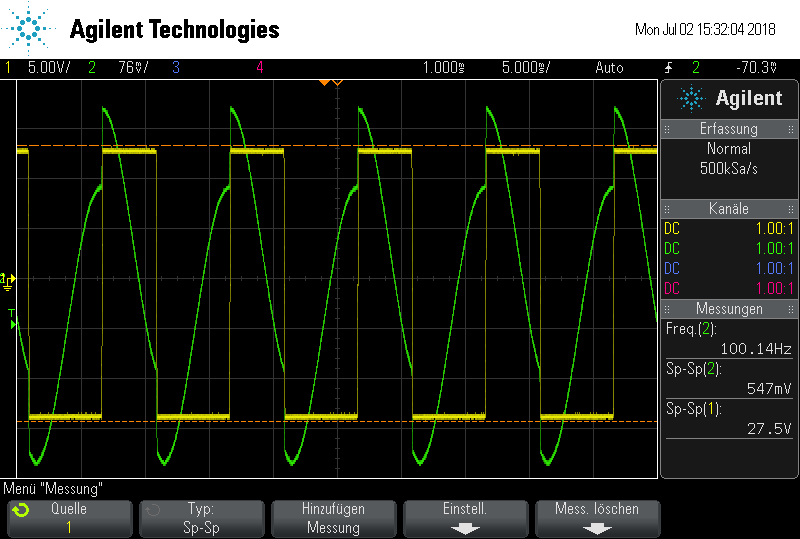
\includegraphics[height=0.3\textheight]{data/scope_268.png}
    \caption{Aufnahmen des Oszilloskops.}
    \label{fig:schmitt_osz}
  \end{subfigure}
  \begin{subfigure}{\textwidth}
    \centering
    \input{build/schmitt.pgf}
    \caption{Oszilloskopdaten mit markierter Schwelle der Sinuseingangsspannung.}
    \label{fig:schmitt_plot}
  \end{subfigure}
  \caption{Messwerte des Schmitt-Triggers.}
  \label{fig:schmitt}
\end{figure}

\subsection{Dreieckgenerator}
Ein Dreieckgenerator wird mit den Bauteilen
$C = \SI{20.8}{\nano\farad}$,
$R_1 = \SI{0.1}{\kilo\ohm}$,
$R_\text{P} = \SI{1}{\kilo\ohm}$,
$R = \SI{30.2}{\kilo\ohm}$
gebaut.
In Abbildung~\ref{fig:dreieck_generator} wird ein Oszilloskopbild
der Ausgangsspannung des Dreieckgenerators dargestellt.
\begin{figure}[ht]
  \centering
  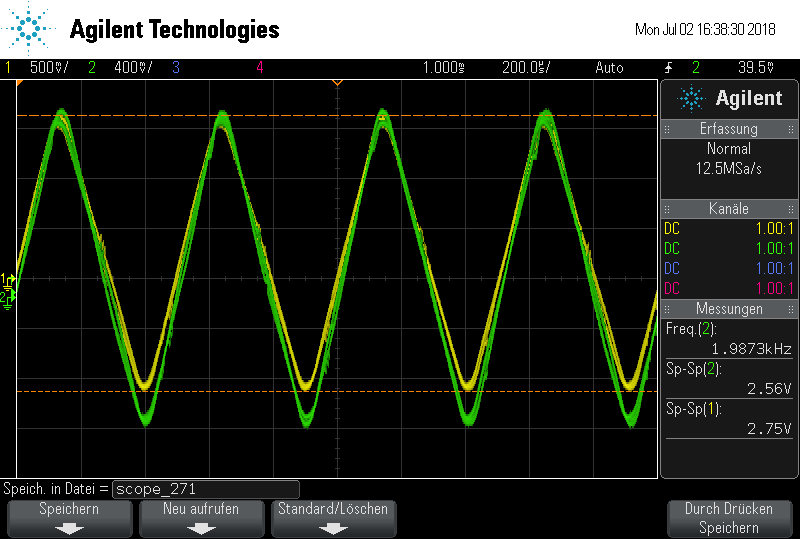
\includegraphics[height=0.3\textheight]{data/scope_271.png}
  \caption{Oszilloskopaufnahme des Dreieckgenerators.}
  \label{fig:dreieck_generator}
\end{figure}

Die Frequenz und Amplitude der Dreieckspannung werden am Oszilloskop abgelesen:
\begin{align*}
  \nu &= \SI{1.99}{\kilo\hertz} \\
  A &= \SI{1.37}{\volt}
\end{align*}

\subsection{Ged\"ampfte Schwingung}
% =================================

\begin{figure}[ht]
  \centering
  \begin{subfigure}{\textwidth}
    \centering
    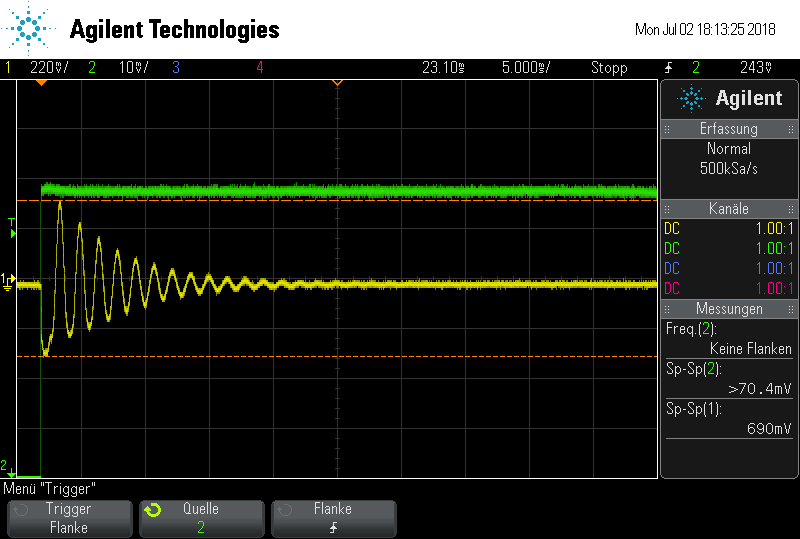
\includegraphics[height=0.3\textheight]{data/scope_275.png}
    \caption{Aufnahme des Oszilloskops.}%
    \label{fig:gedaempft_oszilloskop}
  \end{subfigure}
  \begin{subfigure}{\textwidth}
    \centering
    \input{build/gedaempfte_schwingung.pgf}
    \caption{Oszilloskopdaten mit Fit.}%
    \label{fig:gedaempft_fit}
  \end{subfigure}
  \caption{Messwerte und Fit der gedämpften Schwingung.}%
  \label{fig:gedaempft}
\end{figure}

Die Betriebsspannung wird auf $U_B = \pm \SI{1.95}{\volt}$ gestellt.
Die gedämpfte Schwingung ist in Abbildung~\ref{fig:gedaempft} dargestellt.
Es wird ein Fit der Form
\begin{equation}
  % U = \log{\left(x\right)} \cdot m + b
U = U_0 \cdot \exp{\left(\frac{-t}{\tau}\right)} \cdot \sin{\left(t \cdot \omega  + \phi\right)} + b
\end{equation}
in einem logarithmischen Diagramm (vgl. Abbildung~\ref{fig:gedaempft_fit}) aufgetragen.
Die Parameter des Fits sind
\begin{align*}
  U_0 &= \SI{-0.463 \pm 0.005}{\volt} \\
  \omega &= \SI{4260.068 \pm 2.527}{\kilo\hertz} \\
  \tau &= \SI{0.0047 \pm 0.0001}{\second} \\
  b &= \SI{-0.023 \pm 0.004}{\volt} \\
  \phi &= \SI{-8.075 \pm 0.01}{\radian}.
\end{align*}
Daraus ergeben sich nach Gleichung~\eqref{eq:schwingung_diff} und~\eqref{eq:tau}
\begin{align*}
  \Delta \omega &= \num{11.39}\% \\
    \Delta \tau &= \num{12.05}\%.
\end{align*}
